\documentclass[a4paper,fontset=mac]{ctexart}
\linespread{1.5}                         %行距
\usepackage[top=2cm,bottom=2cm,left=2.5cm,right=2.5cm]{geometry}
% \headsep=2cm
% \textwidth=16cm \textheight=24.2cm
\usepackage{fontspec,xltxtra,xunicode}
\usepackage[colorlinks,linkcolor=blue,anchorcolor=red,citecolor=green,urlcolor=blue]{hyperref}  
\usepackage{tabularx}
\usepackage{amsmath}                   % 数学符号与公式
\usepackage{amsfonts}                  % 数学符号与字体
\usepackage{graphics}
\usepackage{subfigure}
\usepackage{color}
\usepackage{fancyhdr}                  % 设置页眉页脚
\usepackage{fancyvrb}                  % 抄录环境
\usepackage{float}                     % 管理浮动体
\usepackage{geometry}                  % 定制页面格式
\usepackage{hyperref}                  % 为PDF文档创建超链接
\usepackage{lineno}                    % 生成行号
\usepackage{listings}                  % 插入程序源代码
\usepackage{multicol}                  % 多栏排版
\usepackage{rotating}                  % 旋转文字,图形,表格
\usepackage{subfigure}                 % 排版子图形
\usepackage{indentfirst}               % 首段缩进
\usepackage{booktabs}                  % 使用\multicolumn
\usepackage{multirow}                  % 使用\multirow
\usepackage{graphicx}  
\usepackage{xcolor}
\usepackage{cite}
\usepackage{listings}



\lstset{ %
	backgroundcolor=\color[RGB]{245,245,244},   % choose the background color; you must add \usepackage{color} or \usepackage{xcolor}
	basicstyle=\footnotesize,        % the size of the fonts that are used for the code
	breakatwhitespace=false,         % sets if automatic breaks should only happen at whitespace
	breaklines=true,                 % sets automatic line breaking
	captionpos=bl,                    % sets the caption-position to bottom
	commentstyle=\color[RGB]{0,96,96},    % comment style
	deletekeywords={...},            % if you want to delete keywords from the given language
	escapeinside={\%*}{*)},          % if you want to add LaTeX within your code
	extendedchars=true,              % lets you use non-ASCII characters; for 8-bits encodings only, does not work with UTF-8
	frame=none,                    % adds a frame around the code
	keepspaces=true,                 % keeps spaces in text, useful for keeping indentation of code (possibly needs columns=flexible)
	keywordstyle=\color[RGB]{40,40,255},       % keyword style
	%language=Python,                 % the language of the code
	morekeywords={*,...},            % if you want to add more keywords to the set
	numbers=left,                    % where to put the line-numbers; possible values are (none, left, right)
	numbersep=5pt,                   % how far the line-numbers are from the code
	numberstyle=\tiny\color{gray}, % the style that is used for the line-numbers
	rulecolor=\color{black},         % if not set, the frame-color may be changed on line-breaks within not-black text (e.g. comments (green here))
	showspaces=false,                % show spaces everywhere adding particular underscores; it overrides 'showstringspaces'
	showstringspaces=false,          % underline spaces within strings only
	showtabs=false,                  % show tabs within strings adding particular underscores
	stepnumber=1,                    % the step between two line-numbers. If it's 1, each line will be numbered
	stringstyle=\color[RGB]{128,0,0},     % string literal style
	tabsize=2,                       % sets default tabsize to 2 spaces
	language=c++,
	%title=myPython.py                   % show the filename of files included with \lstinputlisting; also try caption instead of title
}


\graphicspath{{sources/}}
\setlength{\parindent}{2em}       %设置缩进为两个大写M的宽度,大约为两个汉字的宽度
\ctexset{section = {format = \raggedright\Large\bfseries,}} %section 左对齐
\graphicspath{{sources/}}


%------------------------------设置字体大小------------------------%  
\newcommand{\cuhao}{\fontsize{42pt}{\baselineskip}\selectfont}     %初号  
\newcommand{\xiaocuhao}{\fontsize{36pt}{\baselineskip}\selectfont} %小初号  
\newcommand{\yihao}{\fontsize{28pt}{\baselineskip}\selectfont}      %一号  
\newcommand{\erhao}{\fontsize{21pt}{\baselineskip}\selectfont}      %二号  
\newcommand{\xiaoerhao}{\fontsize{18pt}{\baselineskip}\selectfont}  %小二号  
\newcommand{\sanhao}{\fontsize{15.75pt}{\baselineskip}\selectfont}  %三号  
\newcommand{\sihao}{\fontsize{14pt}{\baselineskip}\selectfont}       %四号  
\newcommand{\xiaosihao}{\fontsize{12pt}{\baselineskip}\selectfont}  %小四号  
\newcommand{\wuhao}{\fontsize{10.5pt}{\baselineskip}\selectfont}    %五号  
\newcommand{\xiaowuhao}{\fontsize{9pt}{\baselineskip}\selectfont}   %小五号  
\newcommand{\liuhao}{\fontsize{7.875pt}{\baselineskip}\selectfont}  %六号  
\newcommand{\qihao}{\fontsize{5.25pt}{\baselineskip}\selectfont}    %七号


\setCJKmainfont[BoldFont={STHeiti}, ItalicFont={STKaiti}]{STSong}
%\setCJKsansfont{SimHei}
\setCJKsansfont{STHeiti}
%\setCJKmonofont{FangSong}
\setCJKmonofont{STFangsong}

\setmainfont{Times New Roman}   %西文默认衬线字体(serif)
\setsansfont{Arial}   %西文默认无衬线字体(sans serif)
\setmonofont{Courier New}           %西文默认的等宽字体




\title{STL阅读笔记}
\author{sharwen}
\date{}
%==================================================
%%%%%%%%%%%%%%%%%%%%%%%%%%%%%%%%%%%%%%%%%%%%%%%%%%%
% 正文
%==================================================
\begin{document}
	% \pagenumbering{Roman}          %页码为大写罗马数字
	% \pagenumbering{arabic}         %页码为阿拉伯数字
%	{\tiny \thispagestyle{empty}   %本页不显示页码
%	\begin{figure}[h]
%		\centering
%		
\includegraphics[width=5in]{logo1}
%		
\includegraphics[width=2in]{logo2}
%	\end{figure}
%	
%	\vspace{42pt}
%	\begin{table}[h]
%		\centering
%		\linespread{2}   
%		\sanhao
%		\begin{tabular}{lcl}% 通过添加 | 来表示是否需要绘制竖线
%		%		\hline  % 在表格最上方绘制横线
%		\textbf{题\, \; \; \; 目}&\textbf{:}&\textbf{论文综述题目}\\
%		\textbf{姓名学号}&\textbf{:}&\textbf{罗胜文/21821167}\\
%		\textbf{邮\, \; \; \; 箱}&\textbf{:}&\textbf{sharwen568@gmail.com}\\
%		\textbf{电\, \; \; \; 话}&\textbf{:}&\textbf{18883287841}\\
%		\textbf{老\, \; \; \; 师}&\textbf{:}&\textbf{。。。}\\
%		\textbf{专\, \; \; \; 业}&\textbf{:}&\textbf{计算机科学与技术}\\
%		\end{tabular}
%	
%		\vspace{42pt}
%		\centering
%		\textbf{2019年1月9日}
%	\end{table}
%	
%
%	\newpage
%	\setcounter{page}{1}}
	\maketitle
	\tableofcontents
%	\begin{abstract}
%		abstract goes here.
%		
%		\centering%使得关键字居中
%		\textbf{关键字:}摘要、\LaTeX、中文
%	\end{abstract}
	\newpage%另起一页
	
	\section{allocator}
		allocator是STL模板的基础,主要承载工作分为三个方面:1、内存分配;2、对象构造;3、对象析构;4、数据初始化;5、内存回收。
		\subsection{内存分配}
			allocator内存分配为层次内存分配,在SGI-STL源码中,为两级内存分配:第一级配置器使用场景为一次分配内存$\color{red}{More \; Than\;}\boldsymbol{128BYTE}$即超过128字节时,使用第一级内存配置器;第二级配置是一次分配内存$\color{red}{Less \; Than\;}\boldsymbol{128BYTE}$即少于128字节时,使用第二级配置器。使用两级配置器的目的是尽量减少内存碎片化的问题。
		
		\subsubsection{第一级配置器}
			第一级配置内存分配是对malloc,realloc,calloc和free的再次封装,因为这些函数是C语言的内存操作函数,不自带类似C++ set\_new\_handler,因此STL为对内存分配失败加入了类似C++的new\_hander处理机制,允许客户端自己设定内存分配失败的处理函数。内存分配失败处理body是个for循环函数,如下:
			\begin{lstlisting}
			// 不断尝试释放、配置
			for (;;) {
				__my_malloc_handler = __malloc_alloc_oom_handler;
				if (0 == __my_malloc_handler) { __THROW_BAD_ALLOC; }   
					(*__my_malloc_handler)();  // 调用处理例程,企图释放内存
					__result = malloc(__n);   // 再次尝试配置内存
				if (__result) return(__result);
			}
			\end{lstlisting}
			
		\subsubsection{第二级配置器}
		第二级配置器是allocator内存分配的精髓,为了降低内存碎片化问题,STL将申请一个内存pool用作小块内存的分配回收和管理。第一级配置器维护$\bold{\color{red}{16 = MAX\_SIZE / 8}}$个空闲内存链表,其中MAX\_SIZE = 128。
		
		index从0开始。空闲链表分别代表$\color{blue}{chunk \; size\;}$为8,16,24,32,40,48,56,64,72,80,88,96,104,112,120,128。分配会根据请求分配内存的大小,决定从对应的free\_list中分配空闲内存。index = \_S\_round\_up(size) / 8;在内存对齐上,有一个有意思的写法,灵活利用了位运算(ALIGN = 8)。
		
		\begin{lstlisting}
			// 将任何小额区块的内存需求量上调至 8 的倍数
			static size_t
			_S_round_up(size_t __bytes)
			{ return (((__bytes) + (size_t) _ALIGN-1) & ~((size_t) _ALIGN - 1)); }
		\end{lstlisting}
		
		
		第二级内存配置器的基本思想,分为:
		
		1、如果申请内存大小向8对齐后对应的free\_list中存在空闲内存,则将内存返回给客户端使用;
		
		2、如果1中不存在空闲内存,则调用\_S\_refill函数申请内存,默认申请大小为$\boldsymbol{20}$*size,其中size为内存客户端申请大小向8对齐后的大小,如果申请块$\boldsymbol{equal\;1}$,则直接返回给客户端使用,如果返回的$\boldsymbol{greater \; than 1}$,则第一块给客户端,剩下的块添加对size对应的free\_list链表中;
		
		3、\_S\_chunk\_alloc,是第二级内存分配的核心,维护一个通过malloc申请的heap内存,第二步是调用此函数进行内存分配。此函数内存分陪时候会存在以下情况。
		
		1)如果申请大小(20*size)$\boldsymbol{Less Than}$heap中内存总额大小,则直接将start起始内存返回,并更新heap 的start位置。
		
		2)如果heap内存总额大小$\boldsymbol{Less than}$ 20 * size但是够一个以上内存块的分配,则分配最大块数给调用者,余下的内存保留在维护的heap当中。
		
		3)如果一块内存都不够分配,则将heap中的内存挂载到heap内存大小对应的free\_list当中。并进行下一步计算本次内存申请大小:注意此次申请大小为2倍上层调用的大小+总heap大小偏移>>4的总和,此函数调用次数的增加会上升每次申请大小的偏移大小。
		\begin{lstlisting}
		//_S_heap_size是内存配置器维护的heap总申请大小
		size_t __bytes_to_get = 2 * __total_bytes + _S_round_up(_S_heap_size >> 4); 
		...
		_S_heap_size += __bytes_to_get;
		\end{lstlisting}
		
		此时尝试直接用malloc申请内存,如果申请成功,则递归调用\_S\_chunk\_alloc更新成功申请内存的块数量。
		如果失败,则尝试是否能从已有的free\_list中找到可用的内存,进行以下步骤:
		
		a)从申请内存块对应的free\_list索引开始,循环查找free\_list中是否存在空闲的内存块,如果存在,则递归调用自己更新heap指针和申请成功的内存块大小。
		
		b)如果free\_list中不存在,则调用一级配置器,寄希望于malloc和new\_hander,如果成功递归调用自己更新heap指针和申请成功块大小,如果均失败,则抛出失败异常。
		
		在第二级配置中,STL巧妙利用了联合体来管理空闲内存,对配置起数据就是空闲内存块链表指针,对客户端来讲看到的就是真实的数据。
		\begin{lstlisting}
		union _Obj {
			union _Obj* _M_free_list_link;
			char _M_client_data[1];    /* The client sees this.        */
		};
		\end{lstlisting}
		
		
		\subsection{对象构造}
		对象构造没什么好说的,仅仅是对C++ operator new的封装。见图\ref{STL_Constructor}。
		
		
		
		\subsection{对象析构}
		对象析构主要分为两部分,分为两部分的标准是看对象是否存在$\boldsymbol{trivial\; deconstructor}$,首先接受以下trivial deconstructor的含义,指的是对象使用默认析构函数,无自定义析构函数。见图\ref{STL_Constructor}。
		
		对于使用默认析够函数的对象,allocator为了提升效率,啥也不做。
		
		对于自定义析够函数的对象,allocator通过循环一个一个对象调用对象的析够函数进行析够。
		\begin{figure}
			\centering
			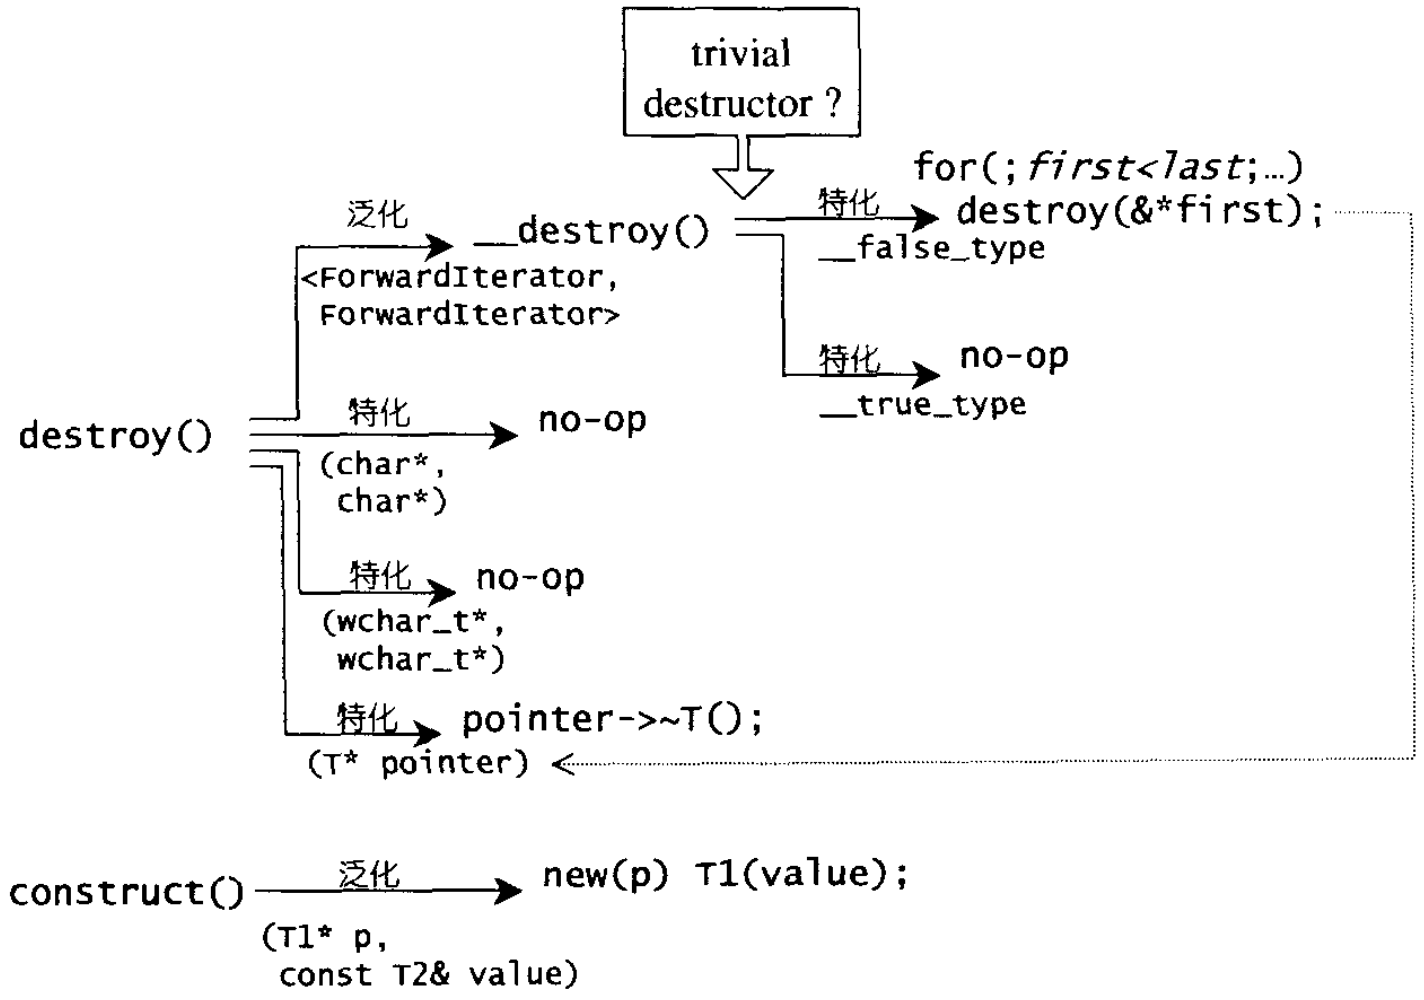
\includegraphics[width=4in]{STL_de_constructor}
			\caption{STL constructor deconstructor example}
			\label{STL_Constructor} %% label for entire figure
		\end{figure}
		
		\subsection{数据初始化}
		数据初始化主要包括uninitialized\_copy,uninitialized\_copy\_n,uninitialized\_fill,uninitialized\_fill\_n函数,这些函数核心都在于区分对象是否为$\boldsymbol{is\_POD\_type}$(pod,Plain Old Data),
		
		如果是POD\_type,则直接使用STL中的copy或者fill模版;
		
		如果不是POD\_type,则利用循环依次对[start\_iterend\_iter)进行对象构造
		
		\subsection{内存回收}
		内存回收和内存分配同样分为两级,
		
		当回收内存向上对8对齐后,如果大于128byte,直接利用free;
		当回收内存向上对8对齐后,小于等于128byte,则作为free block挂载到对应的free\_list索引链表当中去。
		
	
		\section{迭代器与traits}
		\subsection{迭代器分类}
		迭代器分为五类:
		
		1、Input Iterator(只读)
		
		2、Output Iterator(只写)
		
		3、Forward Iterator
		
		4、bidirectional iterator
		
		5、random access iterator
		
		前三类迭代器支持operator++,第四种外加支持operator--,第五种除了前两种operator外,同时支持指针算术运算能力。如图\ref{iterator classify and inherit relationships}
		\begin{figure}
			\centering
			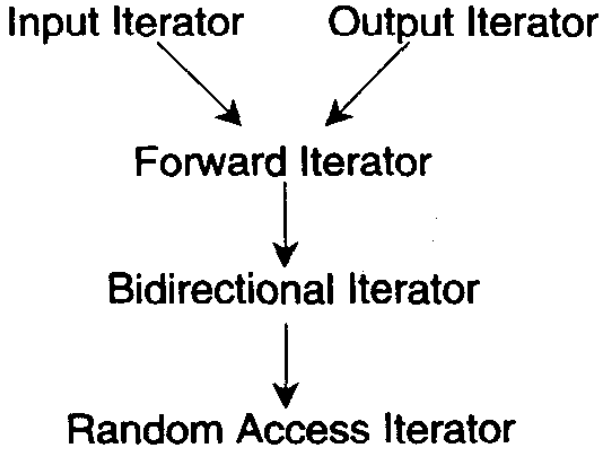
\includegraphics[width=1.5in]{iterator_classify}
			\caption{iiterator\_classify and inherit relationships}
			\label{iterator classify and inherit relationships} %% label for entire figure
		\end{figure}
	
	\subsection{traits判断POD}
	为了提升效率,SGI-STL包含了非标准的特性,通过判断特定属性来决定模板的重载:
	\begin{lstlisting}
	template <class _Tp>
	struct __type_traits { 
		typedef __true_type     this_dummy_member_must_be_first;
		
		typedef __false_type    has_trivial_default_constructor;
		typedef __false_type    has_trivial_copy_constructor;
		typedef __false_type    has_trivial_assignment_operator;
		typedef __false_type    has_trivial_destructor;
		typedef __false_type    is_POD_type;
	};
	\end{lstlisting}
	对于POD类型,SGI-STL对其进行了特化,五个成员均定义为\_\_true\_type,如:
	\begin{lstlisting}
	__STL_TEMPLATE_NULL struct __type_traits<char> { //__STL_TEMPLATE_NULL 为 template<>
		typedef __true_type    has_trivial_default_constructor;
		typedef __true_type    has_trivial_copy_constructor;
		typedef __true_type    has_trivial_assignment_operator;
		typedef __true_type    has_trivial_destructor;
		typedef __true_type    is_POD_type; 
	};
	\end{lstlisting}
	
	\section{序列容器}
	\subsection{vector}
	vector内存空间策略:{\color{red}连续线性}内存空间,与$\boldsymbol{array}$的区别是可以{\color{red}动态分配}内存;
	
	vector内存分配:a)如果插入position内存不足,则以以前的{\color{red}元素个数的两倍空间}申请新内存,然后将原来的数据:1)uninitialized\_copy  begin-position;2)construct(position,val);3)uninitialized\_copy position - finish;4)将原来占用的内存空间返还给系统。
	
	vector erase策略:1)删除迭代器区间范围(start-last),将last-finish copy 到start开始处,然后将copy返回的迭代器i,到finish给destroy掉,同时更新大小。2)删除一个元素position,直接copy position+1 - finish到position处,然后destroy掉finish-1处的元素,更新大小。因此时间复杂度{\color{red}O(N)};
	
	vector insert策略:1)如果剩余的空间满足插入元素个数,如果插入位置position的位置之后的元素大于插入元素个数,则a)将最后n个元素uninitialized\_copy 到finish开始处(因为之后的元素没有构造,所以uninitialized\_copy),b)copy\_backward position - (finish-n)到old\_finish开始处,最后fill掉n个元素到position开始处;如果剩余个数小于插入个数,a)unitialized\_fill\_n 多余的元素;b)将position-old-finish位置的元素unitialized\_copy position - old\_finish到finish开始处,c)fill postion-old\_finish。2) 如果内存不够,则按照vector内存分配进行操作。因此时间复杂度为{\color{red}O(N)}。
	
	vector iterator 实际就是{\color{red}value\_type*},是一个random access iterator。
	
	
	\subsection{list}
	list是一个双向链表,有一个重要的性质,就是{\color{red}插入和删除不会影响除了被删除的迭代器外其余的迭代器仍然有效}。同时list是一个环双向链表,有一个空白end(),可以通过一个指针按照同一方向遍历玩整个链表。
	
	list是一个bidirectional\_iterator;
	
	list是动态申请内存,因此不存在vector的扩容问题,但是也失去了随机访问的能力。
	
	\subsection{deque}
	deque也是动态申请内存,但是与list不同,他的迭代器是一个个random access iterator。
	
	deque内存分配,如图\ref{deque memory allocate}所示。
	\begin{figure}
		\centering
		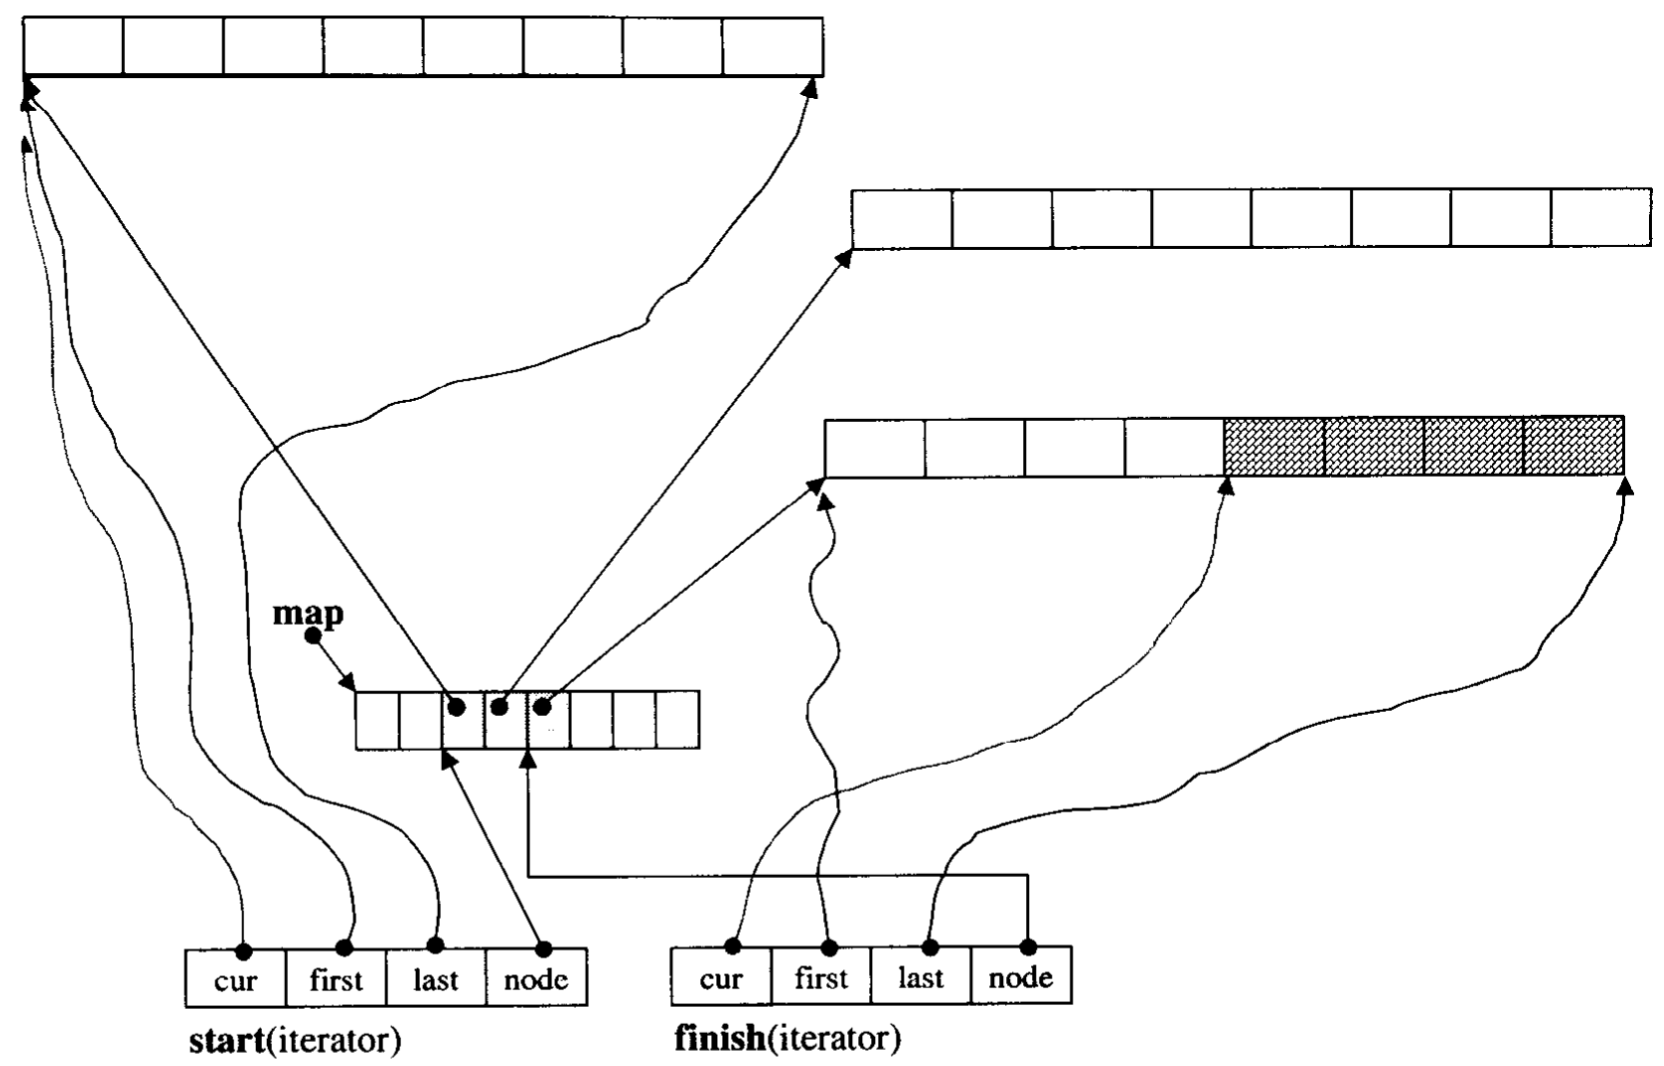
\includegraphics[width=5in]{deque_alloc_memery}
		\caption{deque memory allocate}
		\label{deque memory allocate} %% label for entire figure
	\end{figure}
	
	deque的内存组织,分为两部分,一个中控,为value\_type **,其余是数据存储部分,buffer\_size一般固定,默认512。随机访问迭代器是通过计算的方式实现的,而不是向vector那种天生支持算术运算。
	
	deque的map分配策略,由于deque两端都能够插入或者删除,map分配出现在插入的情况,有一种极端情况就是频繁只在一段插入数据,这会导致另一段的map不怎么使用,这种情况如果频繁插入一端map没空间了,则重新在原map上调整起始位置,移动map映射的位置。map\_size > 2*new\_colum\_num,就会搬运映射而不是重新分配空间。如果不满足这个条件,则重新分配一块风大的空间 new\_map\_size = map\_size + max(map\_size,nodes\_to\_add) + 2,然后将原来的映射拷贝到新map的中间位置。
	
	deque在插入和erase的时候,移动元素会判断前面和后面元素的多少,移动元素少的方向。
	
	\subsection{stack}
	stack是默认使用deque作为底层存储容器,去掉了deque的前端操作,只保留了尾部的操作。
	
	stack没有迭代器。
	
	stack能够手动指定底层容器。
	\subsection{queue}
	queue默认使用deque作为底层容器,而不使用deque的push\_front和pop\_back函数调用,形成FIFO。
	
	queue没有迭代器。
	
	queue能够手动指定底层容器。
	
	\subsection{priority\_queue}
	priority\_queue 底层使用大/小顶堆作为数据处理方式,默认容器为vector
	
	priorty\_queue也不提供迭代器。
	
	\subsection{slist}
	slist是一个单向链表,只能在头部插入,即push\_front,因此只提供单项迭代器operator++。
	
	
	\section{关联式容器}
	\subsection{RB Tree}
	red-black tree 的定义:是平衡二叉搜索树的一种,需要满足以下条件:
	
	1、节点只有red 和 black
	
	2、根结点是black
	
	3、如果节点是red,则子节点一定是black
	
	4、任一节点到NULL(树端点)的任何路径,black节点数量相等
	
	\subsection{set}
	底层容器是红黑树,自动排序,key为const不可修改。
	
	set由于底层采用的是红黑树,因此删除迭代器不会影响其他迭代器,除了被删除的迭代器。
	
	set使用红黑树的insert\_unique接口,因此不允许有重复键值。
	
	\subsection{map}
	map底层同样是红黑树,元素为pair,键值不可修改,但是second值可以修改
	
	map由于底层采用的是红黑树,因此删除迭代器不会影响其他迭代器,除了被删除的迭代器。
	
	map使用红黑树的insert\_unique接口,因此不允许有重复键值。
	
	\subsection{multiset}
	multiset使用红黑树的insert\_equal接口,允许相同的键值存在,其余特性与set相同。
	
	\subsection{multimap}
	multimap使用红黑树的insert\_equal接口,允许相同的键值存在,其余特性与map相同。
	
	\subsection{hash\_table}
	STL hash\_table采用的方式是 {\color{red}桶+开链}方式。
	
	虽然开练法不需要要求table大小为质数,但是STL中还是将表设置为质数大小。
	\begin{lstlisting}
	static const unsigned long __stl_prime_list[__stl_num_primes] =
	{
		53ul,         97ul,         193ul,       389ul,       769ul,
		1543ul,       3079ul,       6151ul,      12289ul,     24593ul,
		49157ul,      98317ul,      196613ul,    393241ul,    786433ul,
		1572869ul,    3145739ul,    6291469ul,   12582917ul,  25165843ul,
		50331653ul,   100663319ul,  201326611ul, 402653189ul, 805306457ul, 
		1610612741ul, 3221225473ul, 4294967291ul
	};
	\end{lstlisting}
	
	\subsubsection{hash\_table内存分配策略}
	 STL中hash\_table内存配置,backet使用的vector容器,开链没有使用list或者deque或者slist,而是自维护一个single\_forward\_link。
	 
	 hash\_table扩桶原则:
	 \begin{lstlisting}
	 const size_type __old_n = _M_buckets.size();
	 if (__num_elements_hint > __old_n) {
		 const size_type __n = _M_next_size(__num_elements_hint);
			 if (__n > __old_n) {
			 	vector<_Node*, _All> __tmp(__n, (_Node*)(0),
			 	_M_buckets.get_allocator());
			 	__STL_TRY {
			 	for (size_type __bucket = 0; __bucket < __old_n; ++__bucket) {
			 	_Node* __first = _M_buckets[__bucket];
			 	while (__first) {
			 		size_type __new_bucket = _M_bkt_num(__first->_M_val, __n);
					 _M_buckets[__bucket] = __first->_M_next;
					 __first->_M_next = __tmp[__new_bucket];
			 		__tmp[__new_bucket] = __first;
			 		__first = _M_buckets[__bucket];          
			 	}
			 }
			 _M_buckets.swap(__tmp);
		 }
	 \end{lstlisting}
	 判断hash\_table中存在的元素个数+1是否大于桶的数量,如果大于则扩容。即判断装载因子是否大于1。分配新的桶后,将以前的元素逐一计算新桶的位置,然后逐一插入。
	 
	 在释放旧桶的时候使用了一个{\color{red}trick},申请一个局部桶,将元素插入到新桶后,利用vector自带的swap交换两个桶,故离开函数后,旧的桶自动释放。
	 
	 hast\_table 插入数据,先找到对应的桶,同时遍历桶中的节点,插入存在两种情况,一不允许插入相同键值(insert\_unique),如果存在相同key的,则返回pair<iterator(cur,this),bool>。否则新建节点头插法插入到桶中,返回pair<iterator(new\_node,this),true>;二是允许插入相同键值(hash\_equal,LLVM中提供的是insert\_multi),同样,首先找桶,然后遍历桶中的元素,如果存在相同的键值,则立马插入,并返回指向new\_node的迭代器,否则新建节点,头插法插入到对应的桶中。这两个接口在后续分别得到hash\_map,hash\_set,和hash\_multimap,hash\_multiset。
	 
	 \subsection{hash\_set}
	 hash\_set使用hash\_table作为底层数据结构,并调用insert\_unique接口。
	 
	 在现在的C++中,hash\_set已经更名为unorderd\_set。
	 
	 \subsection{hash\_map}
	 hash\_map底层使用hash\_table作为底层容器,并调用insert\_unique接口。
	 
	 在现在的C++中,hash\_set已经更名为unorderd\_map。
	 
	 \subsection{hash\_multiset}
	 hash\_multiset使用hash\_table作为底层数据结构,并调用insert\_equal接口。
	 
	 在现在的C++中,STL提供hash版本的multiset 更名为unordered\_multiset。
	 
	 \subsection{hash\_multimap}
	 hash\_multimap使用hash\_table作为底层数据结构,并调用insert\_equal接口。
	 
	 在现在的C++中,STL提供hash版本的multimap 更名为unordered\_multimap。
	 
	 \section{some algorithm}
	 
	 在STL中,通过迭代器得到容器的元素类型其实是强制转换为指针为{\color{red}T*},然后通过模版传入T*,最后在函数中使用真正数据类型T来得到类型变量。
	 \begin{lstlisting}
	 	inline typename iterator_traits<_Iter>::value_type*__value_type(const _Iter&){
		 	return static_cast<typename iterator_traits<_Iter>::value_type*>(0);
	 	}
	 	
	 	
		template <class _ForwardIter1, class _ForwardIter2, class _Tp>
		inline void __iter_swap(_ForwardIter1 __a, _ForwardIter2 __b, _Tp*) {
			_Tp __tmp = *__a;
			*__a = *__b;
			*__b = __tmp;
		}
		
		template <class _ForwardIter1, class _ForwardIter2>
		inline void iter_swap(_ForwardIter1 __a, _ForwardIter2 __b) {
			__STL_REQUIRES(_ForwardIter1, _Mutable_ForwardIterator);
			__STL_REQUIRES(_ForwardIter2, _Mutable_ForwardIterator);
			__STL_CONVERTIBLE(typename iterator_traits<_ForwardIter1>::value_type,
			typename iterator_traits<_ForwardIter2>::value_type);
			__STL_CONVERTIBLE(typename iterator_traits<_ForwardIter2>::value_type,
			typename iterator_traits<_ForwardIter1>::value_type);
			__iter_swap(__a, __b, __VALUE_TYPE(__a));
		}
	 \end{lstlisting}
	 
	 
	 \subsection{copy}
	 copy函数为了优化效率无所不用其极端,copy写了很多特化版本有的直接调用memmove,有的通过赋值运算符,如图\ref{copy}。
	 \begin{figure}
	 	\centering
	 	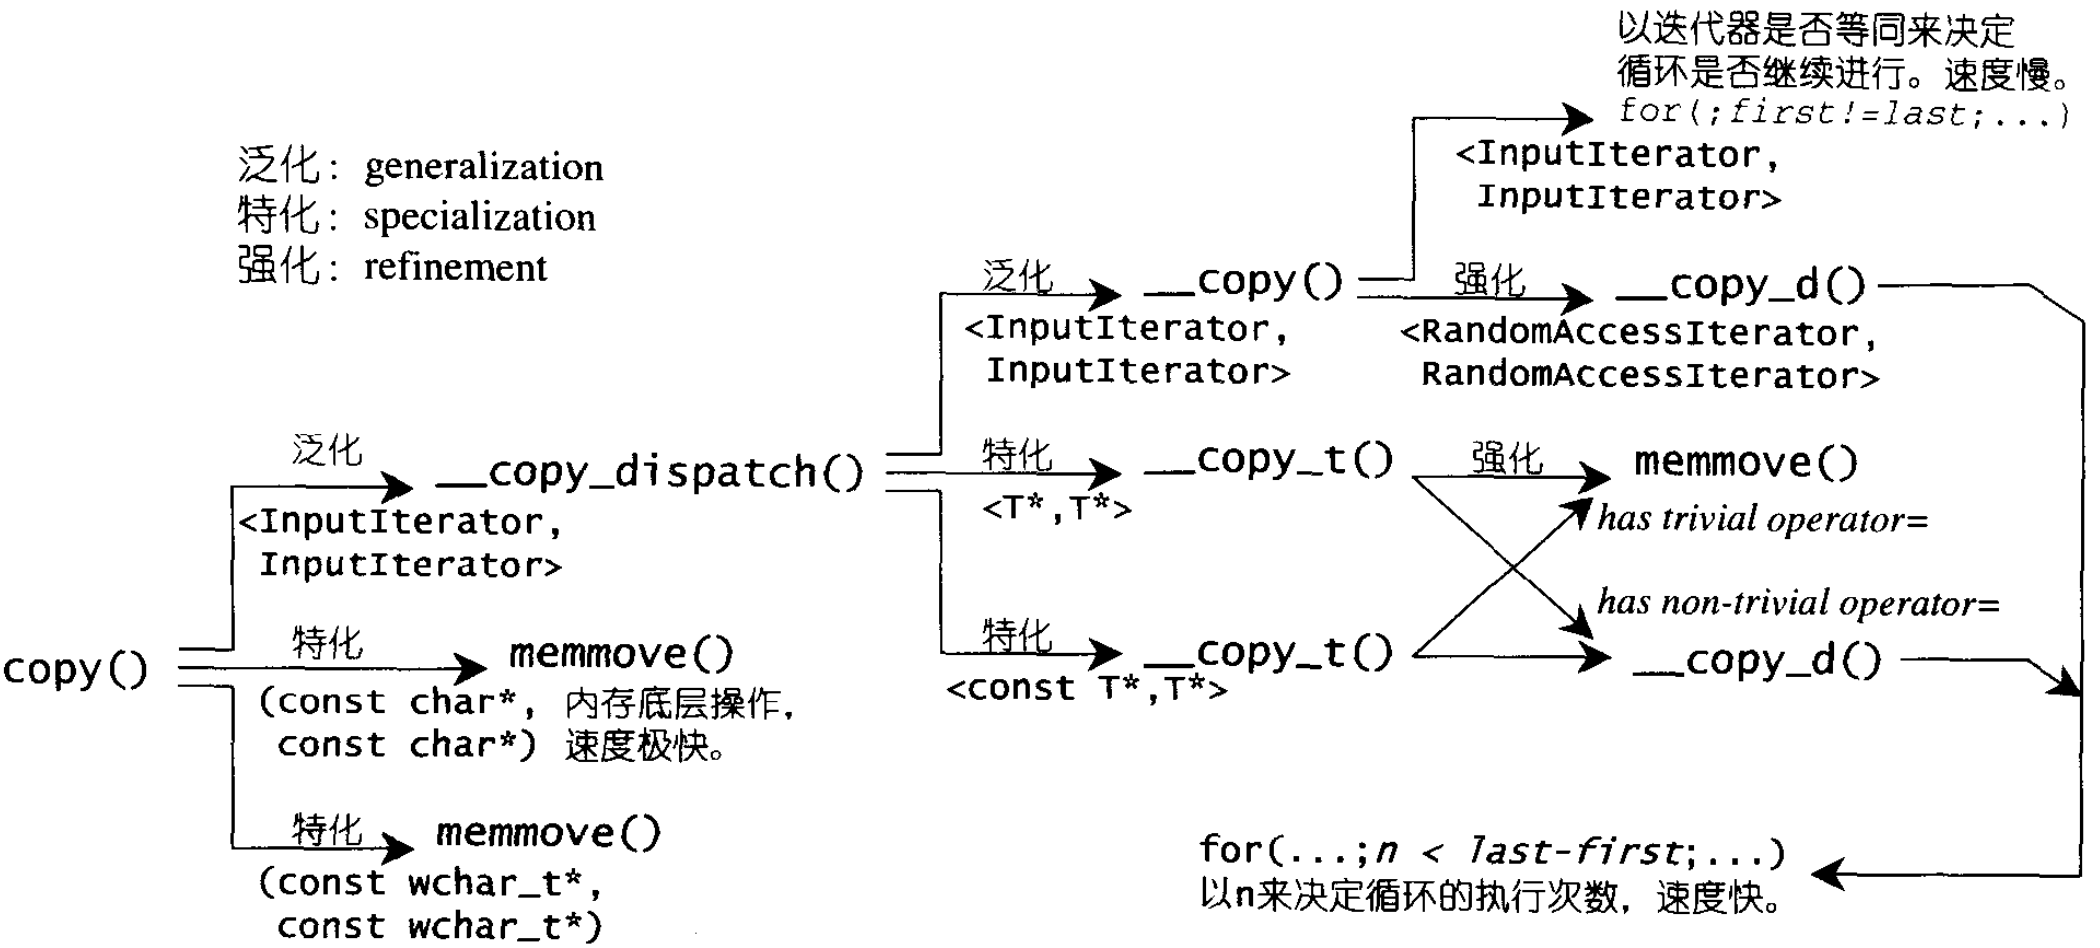
\includegraphics[width=6in]{copy}
	 	\caption{copy}
	 	\label{copy} %% label for entire figure
	 \end{figure}
 
 
 	
 	\section{adapter}
 	配接器的直观解释:扮演转换器的角色,使得原本接口不兼容而不能一起合作的classes,能够一起运作。
 	
 	
	 
	 
	 
	 
	 
	 
	 
	 
	
	
	
	
	
	
	
	
	
	
	
	
	
		
		
		
		
		
		
	
	
	
	
	
	
	
	
	
	
	
	
	
	
	\newpage%另起一页
	\begin{thebibliography}{1}
		\bibitem{STL_book}
		STL源码剖析,侯捷等
	\end{thebibliography}
	
% 插入图片并排,且图片编号不属于同一个大编号,图片编号数字不同
%	\begin{figure}
%		\begin{minipage}[t]{0.5\linewidth}
%			\centering
%			
\includegraphics[width=2.2in]{logo1}
%			\caption{fig1}
%			\label{logo1}
%		\end{minipage}%
%		\begin{minipage}[t]{0.5\linewidth}
%			\centering
%			
\includegraphics[width=2.2in]{logo2}
%			\caption{fig2}
%			\label{logo2}
%		\end{minipage}
%	\end{figure}



% 插入图片并排,图片属于同一个编号,但是每一个图片有自己的子编号a,b,c
%\begin{figure}
%	\centering
%	\subfigure[logo1]{
%		\label{logo1} %% label for first subfigure
%		
\includegraphics[width=1.0in]{logo1}}
%	\hspace{1in}
%	\subfigure[logo2]{
%		\label{logo2} %% label for second subfigure
%		
\includegraphics[width=1.5in]{logo2}}
%	\caption{Two Subfigures}
%	\label{logo} %% label for entire figure
%\end{figure}


	\end{document}
%==================================================
%%%%%%%%%%%%%%%%%%%%%%%%%%%%%%%%%%%%%%%%%%%%%%%%%%%